
%(BEGIN_QUESTION)
% Copyright 2007, Tony R. Kuphaldt, released under the Creative Commons Attribution License (v 1.0)
% This means you may do almost anything with this work of mine, so long as you give me proper credit

Write a minimized (simplest form) Boolean expression for the logic function represented by this truth table, and then sketch both a binary (gate) logic diagram and a ladder logic diagram to implement your simplified Boolean expression:

% No blank lines allowed between lines of an \halign structure!
% I use comments (%) instead, so that TeX doesn't choke.

$$\vbox{\offinterlineskip
\halign{\strut
\vrule \quad\hfil # \ \hfil & 
\vrule \quad\hfil # \ \hfil & 
\vrule \quad\hfil # \ \hfil & 
\vrule \quad\hfil # \ \hfil \vrule \cr
\noalign{\hrule}
%
% First row
Input A & Input B & Input C & Output \cr
%
\noalign{\hrule}
%
% Another row
0 & 0 & 0 & 0 \cr
%
\noalign{\hrule}
%
% Another row
0 & 0 & 1 & 0 \cr
%
\noalign{\hrule}
%
% Another row
0 & 1 & 0 & 1 \cr
%
\noalign{\hrule}
%
% Another row
0 & 1 & 1 & 1 \cr
%
\noalign{\hrule}
%
% Another row
1 & 0 & 0 & 1 \cr
%
\noalign{\hrule}
%
% Another row
1 & 0 & 1 & 0 \cr
%
\noalign{\hrule}
%
% Another row
1 & 1 & 0 & 1 \cr
%
\noalign{\hrule}
%
% Another row
1 & 1 & 1 & 0 \cr
%
\noalign{\hrule}
} % End of \halign 
}$$ % End of \vbox

\underbar{file i02337}
%(END_QUESTION)





%(BEGIN_ANSWER)

$$\includegraphics[width=15.5cm]{i02337x01.eps}$$

$$\includegraphics[width=15.5cm]{i02337x02.eps}$$

\vskip 10pt

Boolean expression = $\overline{A}B + A\overline{C}$

\vskip 10pt

If complete a Karnaugh map for this truth table, you get the following result:

$$
\includegraphics[width=15.5cm]{i02337x03.eps}$$

The best grouping for this map is as follows:

$$\includegraphics[width=15.5cm]{i02337x04.eps}$$

This grouping yields the following (simplified) expression: $\overline{A}B + A\overline{C}$.

\vskip 10pt

One year in class, a student asked what would happen if we made a third group in the Karnaugh map like this:

$$\includegraphics[width=15.5cm]{i02337x05.eps}$$

Now, certainly this new group ($B\overline{C}$) does not contribute anything to the answer other than a redundant term.  However, the remark was made that the new (three-term) expression did not appear to be reducible to the first (two-term) expression:

$$\hbox{Is } \overline{A}B + A\overline{C} \hbox{ the same as } \overline{A}B + A\overline{C} + B\overline{C} \hbox{ ???}$$

\filbreak

It turns out the answer is yes, and it takes the form of a new Boolean reduction rule I was not previously aware of, the general form being:

$$AX + \overline{A}Y + XY = AX + \overline{A}Y$$

Here is the proof, starting with the rule and progressing to show an equality.  My first step is to use the rule $A + AB = A$ to expand two terms on the right-hand side of the equation:

$$AX + \overline{A}Y + XY = (A + AY)X + (\overline{A} + \overline{A}X)Y$$

Next, I distribute:

$$AX + \overline{A}Y + XY = AX + AXY + \overline{A}Y + \overline{A}XY$$

Finally, factoring $XY$ from two of the new terms, and simplifying:

$$AX + \overline{A}Y + XY = AX + \overline{A}Y + XY(A + \overline{A})$$

$$AX + \overline{A}Y + XY = AX + \overline{A}Y + XY(1)$$

$$AX + \overline{A}Y + XY = AX + \overline{A}Y + XY$$

Applying this rule to the three-term SOP expression resulting from the Karnaugh map with the extra group:

$$\overline{A}B + A\overline{C} + B\overline{C}$$

Here, we take $\overline{A}$ to be $A$ in the rule, $B$ to be $X$ in the rule, and $\overline{C}$ to be $Y$ in the rule:

$$\overline{A}B + A\overline{C}$$

%(END_ANSWER)





%(BEGIN_NOTES)


%INDEX% Electronics review: truth table to Boolean expression to logic circuit

%(END_NOTES)


